\documentclass[11pt]{article}

\usepackage[margin=0.72in,bottom=0.82in]{geometry}
\usepackage[T1]{fontenc}
\usepackage{lmodern}
\usepackage{amsmath,amssymb,amsfonts}
\usepackage{array,booktabs,multicol,tabularx}
\usepackage{tikz}
\usepackage[most]{tcolorbox}
\usepackage{xcolor}
\usepackage{fancyhdr}
\usepackage{lastpage}
\usepackage{enumitem}
\usepackage{mathtools}
\usepackage{needspace}
\usepackage{titlesec}
\usepackage{hyperref}

\hypersetup{hidelinks}
\usetikzlibrary{arrows.meta,calc,patterns,positioning}

% =========================
% Novel Prep Brand System
% =========================
\definecolor{npPurple}{RGB}{118,83,255}
\definecolor{npDeep}{RGB}{76,54,180}
\definecolor{npLilac}{RGB}{246,243,255}
\definecolor{npLine}{RGB}{206,196,255}
\definecolor{npInk}{RGB}{31,31,38}
\definecolor{npSoft}{RGB}{250,250,252}
\definecolor{npGray}{RGB}{115,115,128}

\pagestyle{fancy}
\fancyhf{}
\lhead{\textcolor{npDeep}{\textbf{Novel Prep Learning Center}}}
\rhead{\textcolor{npDeep}{\textbf{Middle Level Math Placement}}}
\cfoot{\textcolor{npGray}{Page \thepage\ of \pageref{LastPage}}}
\setlength{\headheight}{15pt}

\setlength{\parindent}{0pt}
\setlength{\parskip}{0.32em}
\renewcommand{\arraystretch}{1.18}

\titleformat{\section}
  {\Large\bfseries\color{npDeep}}
  {}{0pt}{}
  [\vspace{-0.45em}\textcolor{npLine}{\titlerule[0.9pt]}]

\titleformat{\subsection}
  {\large\bfseries\color{npDeep}}
  {}{0pt}{}

% =========================
% Boxes and Commands
% =========================
\newtcolorbox{titlebox}{
  enhanced,
  colback=npLilac,
  colframe=npLine,
  borderline west={3pt}{0pt}{npPurple},
  boxrule=0.65pt,
  arc=2pt,
  left=9pt,right=9pt,top=8pt,bottom=8pt
}

\newtcolorbox{guidebox}{
  enhanced,
  colback=white,
  colframe=npLine,
  boxrule=0.75pt,
  arc=2pt,
  left=9pt,right=9pt,top=8pt,bottom=8pt
}

\newcommand{\ansline}{\rule{2.25in}{0.4pt}}
\newcommand{\work}[1]{\vspace*{#1}}
\newcommand{\blank}{\rule{0.72in}{0.45pt}}
\newcommand{\sectiontag}[1]{%
  \vspace{0.35em}
  {\large\textcolor{npDeep}{\textbf{#1}}}\par
  \vspace{-0.2em}\textcolor{npLine}{\rule{\linewidth}{0.7pt}}\vspace{0.25em}
}

\newcommand{\circnum}[1]{%
\begin{tikzpicture}[baseline=(char.base)]
\node[
  draw=npPurple,
  circle,
  inner sep=1.45pt,
  line width=0.85pt,
  text=npDeep
] (char) {\strut\small\textbf{#1}};
\end{tikzpicture}}

\newcommand{\qnum}[1]{\needspace{3.4\baselineskip}\item[\circnum{#1}]}
\newcommand{\diagramchip}[1]{%
  \node[
    fill=npLilac,
    draw=npLine,
    rounded corners=2pt,
    inner xsep=3.2pt,
    inner ysep=1.1pt,
    line width=0.45pt,
    font=\tiny\bfseries\color{npDeep}
  ] {Q#1};
}

% =========================
% Diagram Helpers
% =========================
\newcommand{\rectmixed}{%
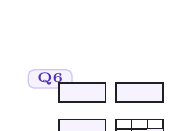
\begin{tikzpicture}[scale=0.44,baseline=-0.5ex]
  \begin{scope}[shift={(-0.25,1.72)}]\diagramchip{6}\end{scope}
  \foreach \x/\y in {0/1.05,1.65/1.05,0/0} {
    \draw[fill=npLilac,draw=npInk,line width=0.65pt] (\x,\y) rectangle ++(1.35,0.55);
  }
  \draw[draw=npInk,line width=0.65pt] (1.65,0) rectangle ++(1.35,0.55);
  \foreach \x in {2.10,2.55}{\draw[draw=npInk,line width=0.45pt] (\x,0)--(\x,0.55);}
  \draw[draw=npInk,line width=0.45pt] (1.65,0.275)--(3.0,0.275);
  \fill[npLilac] (2.55,0) rectangle (3.0,0.275);
\end{tikzpicture}}

\newcommand{\quarterSquare}{%
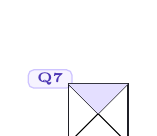
\begin{tikzpicture}[scale=0.42,baseline=-0.5ex]
  \begin{scope}[shift={(-0.55,1.95)}]\diagramchip{7}\end{scope}
  \draw[draw=npInk,line width=0.6pt] (0,0) rectangle (1.8,1.8);
  \draw (0,0)--(1.8,1.8);
  \draw (0,1.8)--(1.8,0);
  \fill[npLine!55] (0,1.8)--(0.9,0.9)--(1.8,1.8)--cycle;
\end{tikzpicture}}

\newcommand{\rectangleSixFour}{%
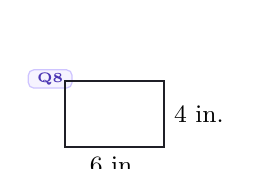
\begin{tikzpicture}[scale=0.42,baseline=-0.5ex]
  \begin{scope}[shift={(-0.45,2.05)}]\diagramchip{8}\end{scope}
  \draw[draw=npInk,line width=0.7pt] (0,0) rectangle (3,2);
  \node[below] at (1.5,0) {\small 6 in.};
  \node[right] at (3,1) {\small 4 in.};
\end{tikzpicture}}

\newcommand{\numberLineTwoEightSix}{%
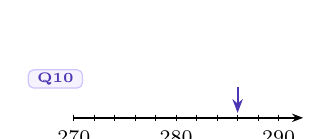
\begin{tikzpicture}[scale=0.52,baseline=-0.5ex]
  \begin{scope}[shift={(-0.45,0.95)}]\diagramchip{10}\end{scope}
  \draw[-{Stealth[length=4pt]},line width=0.55pt] (0,0)--(5.6,0);
  \foreach \i in {0,...,10}{\draw (0.5*\i,0.08)--(0.5*\i,-0.08);}
  \node[below] at (0, -0.08) {\scriptsize 270};
  \node[below] at (2.5, -0.08) {\scriptsize 280};
  \node[below] at (5, -0.08) {\scriptsize 290};
  \draw[-{Stealth[length=5pt]},npDeep,line width=0.8pt] (4.0,0.75)--(4.0,0.12);
\end{tikzpicture}}

\newcommand{\rulerST}{%
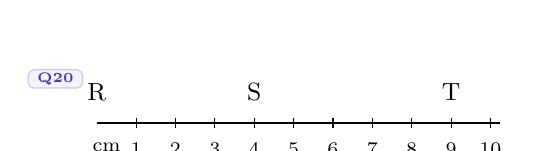
\begin{tikzpicture}[scale=0.5,baseline=-0.5ex]
  \begin{scope}[shift={(-1.05,1.12)}]\diagramchip{20}\end{scope}
  \draw[line width=0.7pt] (0,0)--(10.25,0);
  \foreach \i in {1,...,10}{\draw (\i,0.12)--(\i,-0.12) node[below=2pt] {\scriptsize \i};}
  \node[below=2pt] at (0.25,-0.12) {\scriptsize cm};
  \node[above=3pt] at (0,0.12) {\small R};
  \node[above=3pt] at (4,0.12) {\small S};
  \node[above=3pt] at (9,0.12) {\small T};
\end{tikzpicture}}

\newcommand{\rectRuler}{%
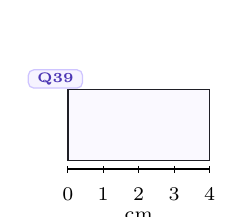
\begin{tikzpicture}[scale=0.45,baseline=-0.5ex]
  \begin{scope}[shift={(-0.35,2.55)}]\diagramchip{39}\end{scope}
  \draw[line width=0.6pt] (0,0)--(4,0);
  \foreach \i in {0,...,4}{\draw (\i,0.1)--(\i,-0.1) node[below=2pt] {\scriptsize \i};}
  \draw[draw=npInk,fill=npLilac!50,line width=0.6pt] (0,0.25) rectangle (4,2.25);
  \node[below=12pt] at (2,0) {\scriptsize cm};
\end{tikzpicture}}

\newcommand{\segmentABC}{%
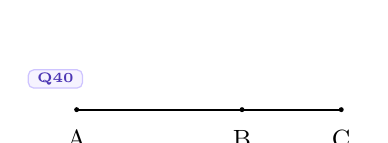
\begin{tikzpicture}[scale=0.6,baseline=-0.5ex]
  \begin{scope}[shift={(-0.45,0.65)}]\diagramchip{40}\end{scope}
  \draw[line width=0.7pt] (0,0)--(5.6,0);
  \foreach \x/\n in {0/A,3.5/B,5.6/C}{\fill (\x,0) circle (1.5pt) node[below=4pt] {\small \n};}
\end{tikzpicture}}

\newcommand{\lShapeArea}{%
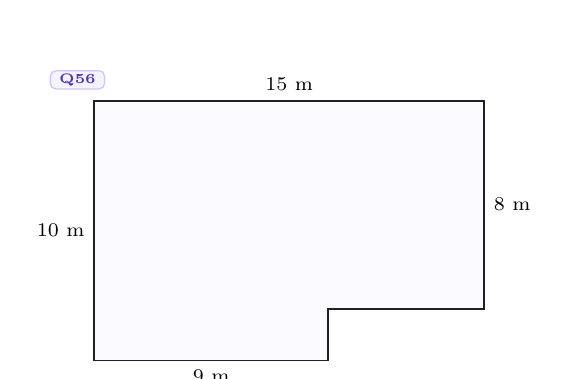
\begin{tikzpicture}[scale=0.33,baseline=-0.5ex]
  \begin{scope}[shift={(-0.65,10.8)}]\diagramchip{56}\end{scope}
  \draw[draw=npInk,fill=npLilac!40,line width=0.7pt] (0,0)--(9,0)--(9,2)--(15,2)--(15,10)--(0,10)--cycle;
  \node[above] at (7.5,10) {\scriptsize 15 m};
  \node[left] at (0,5) {\scriptsize 10 m};
  \node[right] at (15,6) {\scriptsize 8 m};
  \node[below] at (4.5,0) {\scriptsize 9 m};
\end{tikzpicture}}

\newcommand{\pentagonSquare}{%
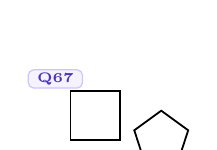
\begin{tikzpicture}[scale=0.48,baseline=-0.5ex]
  \begin{scope}[shift={(-0.40,1.62)}]\diagramchip{67}\end{scope}
  \draw[line width=0.65pt] (0,0) rectangle (1.3,1.3);
  \begin{scope}[shift={(2.4,0.03)}]
    \draw[line width=0.65pt] (90:0.75)--(162:0.75)--(234:0.75)--(306:0.75)--(18:0.75)--cycle;
  \end{scope}
\end{tikzpicture}}

\newcommand{\triPrism}{%
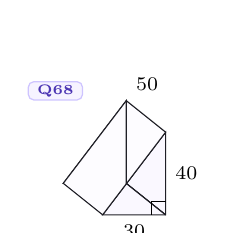
\begin{tikzpicture}[scale=0.5,baseline=-0.5ex]
  \begin{scope}[shift={(-1.20,3.15)}]\diagramchip{68}\end{scope}
  \coordinate (A) at (0,0); \coordinate (B) at (1.6,0); \coordinate (C) at (1.6,2.1);
  \coordinate (D) at (-1.0,0.8); \coordinate (E) at (0.6,0.8); \coordinate (F) at (0.6,2.9);
  \draw[fill=npLilac!55,draw=npInk] (A)--(B)--(C)--cycle;
  \draw[fill=npLilac!35,draw=npInk] (D)--(E)--(F)--cycle;
  \draw[fill=npLilac!25,draw=npInk] (A)--(D)--(F)--(C)--cycle;
  \draw[draw=npInk] (B)--(E)--(F); \draw[draw=npInk] (B)--(E);
  \draw (1.25,0)--(1.25,0.35)--(1.6,0.35);
  \node[right] at (1.6,1.05) {\scriptsize 40};
  \node[below] at (0.8,0) {\scriptsize 30};
  \node[above right] at (0.6,2.9) {\scriptsize 50};
\end{tikzpicture}}

\newcommand{\similarTriangles}{%
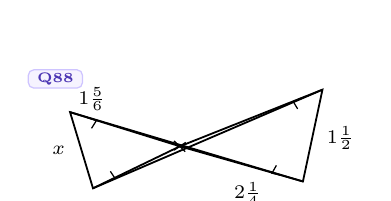
\begin{tikzpicture}[scale=0.62,baseline=-0.5ex]
  \begin{scope}[shift={(-2.55,1.38)}]\diagramchip{88}\end{scope}
  \coordinate (O) at (0,0);
  \coordinate (A) at (-2.25,0.70);
  \coordinate (B) at (-1.78,-0.86);
  \coordinate (C) at (2.92,1.16);
  \coordinate (D) at (2.52,-0.72);
  \draw[line width=0.65pt] (A)--(O)--(B)--cycle;
  \draw[line width=0.65pt] (O)--(C)--(D)--cycle;
  \draw[line width=0.65pt] (A)--(D);
  \draw[line width=0.65pt] (B)--(C);
  \node[left] at ($(A)!0.5!(B)+(-0.14,0)$) {\scriptsize \(x\)};
  \node[above left] at ($(A)!0.42!(O)+(-0.02,0.12)$) {\scriptsize \(1\frac{5}{6}\)};
  \node[below] at ($(O)!0.55!(D)+(0,-0.14)$) {\scriptsize \(2\frac14\)};
  \node[right] at ($(C)!0.53!(D)+(0.10,0)$) {\scriptsize \(1\frac12\)};
  \draw[line width=0.45pt] ($(A)!0.16!(O)$) -- ++(0.18,-0.06) -- ++(-0.10,-0.16);
  \draw[line width=0.45pt] ($(B)!0.16!(O)$) -- ++(0.17,0.06) -- ++(-0.10,0.15);
  \draw[line width=0.45pt] ($(C)!0.15!(O)$) -- ++(-0.16,-0.07) -- ++(0.09,-0.15);
  \draw[line width=0.45pt] ($(D)!0.18!(O)$) -- ++(-0.18,0.04) -- ++(0.09,0.16);
  \draw[line width=0.45pt] ($(O)+(-0.12,0.11)$)--($(O)+(0.11,-0.11)$);
  \draw[line width=0.45pt] ($(O)+(-0.12,-0.08)$)--($(O)+(0.12,0.08)$);
\end{tikzpicture}}

\newcommand{\trapezoidSolid}{%
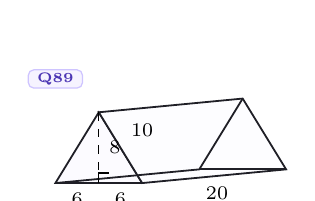
\begin{tikzpicture}[scale=0.58,baseline=-0.5ex]
  \begin{scope}[shift={(0.0,2.28)}]\diagramchip{89}\end{scope}
  \coordinate (A) at (0,0);
  \coordinate (M) at (0.95,0);
  \coordinate (B) at (1.90,0);
  \coordinate (P) at (0.95,1.55);
  \coordinate (s) at (3.15,0.30);
  \coordinate (A2) at ($(A)+(s)$);
  \coordinate (B2) at ($(B)+(s)$);
  \coordinate (P2) at ($(P)+(s)$);
  \draw[fill=npLilac!32,draw=npInk,line width=0.65pt] (A)--(B)--(P)--cycle;
  \draw[fill=npLilac!20,draw=npInk,line width=0.65pt] (B)--(B2)--(P2)--(P)--cycle;
  \draw[draw=npInk,line width=0.65pt] (A)--(A2)--(P2);
  \draw[draw=npInk,line width=0.65pt] (A2)--(B2);
  \draw[dashed,line width=0.5pt] (P)--(M);
  \draw[line width=0.5pt] (M)--++(0,0.22)--++(0.22,0);
  \node[below] at ($(A)!0.5!(M)$) {\scriptsize 6};
  \node[below] at ($(M)!0.5!(B)$) {\scriptsize 6};
  \node[below] at ($(B)!0.52!(B2)+(0,-0.03)$) {\scriptsize 20};
  \node[right] at ($(P)!0.5!(M)+(0.02,0)$) {\scriptsize 8};
  \node[above right] at ($(P)!0.50!(B)+(0.02,0.02)$) {\scriptsize 10};
\end{tikzpicture}}

\newcommand{\baseSolid}{%
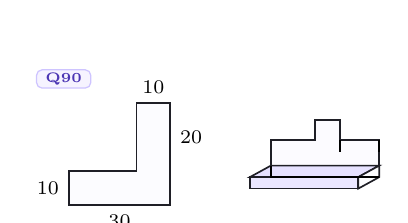
\begin{tikzpicture}[scale=0.43,baseline=-0.5ex]
  \begin{scope}[shift={(-0.15,3.72)}]\diagramchip{90}\end{scope}
  \begin{scope}
    \draw[fill=npLilac!28,draw=npInk,line width=0.65pt]
      (0,0)--(3.0,0)--(3.0,3.0)--(2.0,3.0)--(2.0,1.0)--(0,1.0)--cycle;
    \node[left] at (0,0.5) {\scriptsize 10};
    \node[below] at (1.5,0) {\scriptsize 30};
    \node[above] at (2.5,3.0) {\scriptsize 10};
    \node[right] at (3.0,2.0) {\scriptsize 20};
  \end{scope}
  \begin{scope}[shift={(5.35,0.82)}]
    \coordinate (p0) at (0,0);
    \coordinate (p1) at (3.2,0);
    \coordinate (p2) at (3.2,0.75);
    \coordinate (p3) at (2.05,0.75);
    \coordinate (p4) at (2.05,1.35);
    \coordinate (p5) at (1.30,1.35);
    \coordinate (p6) at (1.30,0.75);
    \coordinate (p7) at (0,0.75);
    \coordinate (v) at (0.62,0.34);
    \coordinate (d) at (0,-0.34);
    \draw[fill=npLilac!32,draw=npInk,line width=0.65pt]
      ($(p0)+(v)$)--($(p1)+(v)$)--($(p2)+(v)$)--($(p3)+(v)$)--($(p4)+(v)$)--($(p5)+(v)$)--($(p6)+(v)$)--($(p7)+(v)$)--cycle;
    \draw[fill=npLine!50,draw=npInk,line width=0.6pt]
      (p0)--(p1)--($(p1)+(v)$)--($(p0)+(v)$)--cycle;
    \draw[fill=npLilac!18,draw=npInk,line width=0.6pt]
      (p1)--($(p1)+(d)$)--($(p1)+(v)+(d)$)--($(p1)+(v)$)--cycle;
    \draw[fill=npLine!42,draw=npInk,line width=0.6pt]
      (p0)--(p1)--($(p1)+(d)$)--($(p0)+(d)$)--cycle;
    \draw[line width=0.6pt] ($(p0)+(v)$)--($(p0)+(v)+(d)$)--($(p1)+(v)+(d)$);
    \draw[line width=0.6pt] ($(p2)+(v)$)--($(p2)+(v)+(d)$);
    \draw[line width=0.6pt] ($(p3)+(v)$)--($(p3)+(v)+(d)$);
  \end{scope}
\end{tikzpicture}}

\newcommand{\longdiv}[2]{%
\begin{tikzpicture}[baseline=-0.55ex]
  \node[anchor=base east] at (0,0) {\(#1\)};
  \draw (0.08,0.38)--(0.08,-0.16)--(1.06,-0.16);
  \node[anchor=base west] at (0.14,0) {\(#2\)};
\end{tikzpicture}}

\newcommand{\verticalmul}[2]{%
\begin{array}{r}
#1\\[-0.12em]
\times\ #2\\ \hline
\end{array}}

\newcommand{\verticaladd}[3]{%
\begin{array}{r}
#1\\[-0.12em]
#2\\ \hline
#3
\end{array}}

\newcommand{\verticalsub}[3]{%
\begin{array}{r}
#1\\[-0.12em]
#2\\ \hline
#3
\end{array}}

\begin{document}

\begin{center}
  {\Large\bfseries\textcolor{npInk}{Novel Prep Learning Center}}\\[0.12cm]
  {\LARGE\bfseries\textcolor{npDeep}{Middle Level Math Placement Test}}\\[0.12cm]
  {\large Math 5 Readiness through Algebra 1 Readiness Diagnostic}\\[0.45cm]
  Name:\ \ansline \hfill Date:\ \ansline
\end{center}

\begin{titlebox}
\textbf{Directions.} Work carefully and show enough work to support your answers. Do not use a calculator unless your instructor allows it. This diagnostic is designed to identify the strongest appropriate starting level: Math 7, Math 8, Algebra 1/2, Algebra 1, or additional advanced assessment.
\end{titlebox}

\begin{guidebox}
\textbf{Teacher Use.} The test is organized in five 20-question bands. A student normally moves to the next readiness band only after scoring at least 16 correct in the current band. Use written work, speed, independence, and error pattern as supporting evidence.
\end{guidebox}

\sectiontag{Part I: Math 5/4 Readiness}
\begin{enumerate}[leftmargin=0pt,itemindent=0pt,labelsep=0.55em,align=left]

\qnum{1} Mae-Ying bought a package of paper priced at \(\$1.98\) and 2 pens priced at \(\$0.49\) each. The tax on the entire purchase was 18 cents. What was the total cost of the items?
\work{1.0cm}

\qnum{2} Seventy-five beans were equally divided into five pots. How many beans were in each pot?
\work{0.9cm}

\qnum{3} Robo could run 7 miles in 1 hour. At that rate, how many miles could Robo run in 3 hours?
\work{0.9cm}

\qnum{4} At 11:45 A.M. Jason glanced at the clock. His doctor's appointment was in \(2\frac12\) hours. At what time was his appointment?
\work{1.0cm}

\qnum{5} Find the sixth number in this counting sequence:
\[
7,\ 14,\ 21,\ \ldots
\]
\work{0.6cm}

\qnum{6} Write the number of shaded rectangles shown as a mixed number. \hfill \rectmixed
\work{0.9cm}

\qnum{7} Twenty-five percent of this square is shaded. What percent of the square is not shaded? \hfill \quarterSquare
\work{0.9cm}

\qnum{8} What is the perimeter of this rectangle? \hfill \rectangleSixFour
\work{1.0cm}

\qnum{9} A square has one side that is 7 inches long. What is the area of the square?
\work{0.9cm}

\qnum{10} To what number is the arrow pointing? \hfill \numberLineTwoEightSix
\work{0.8cm}

\qnum{11} Add:
\[
4.2+3.5+0.25+4.0
\]
\work{0.7cm}

\qnum{12} Multiply:
\[
\verticalmul{460}{9}
\]
\work{0.75cm}

\qnum{13} Divide:
\[
\longdiv{6}{3795}
\]
\work{0.8cm}

\qnum{14} Multiply:
\[
6\times 4\times 10
\]
\work{0.65cm}

\qnum{15} Add:
\[
\begin{array}{r}
\$4.86\\[-0.12em]
+\$2.95\\ \hline
\end{array}
\]
\work{0.7cm}

\qnum{16} Find the missing number:
\[
\begin{array}{r}
z\\[-0.12em]
+179\\ \hline
496
\end{array}
\]
\work{0.75cm}

\qnum{17} Find the missing number:
\[
\begin{array}{r}
67\\[-0.12em]
-B\\ \hline
16
\end{array}
\]
\work{0.75cm}

\qnum{18} Use digits to write the number three hundred forty-three.
\work{0.7cm}

\qnum{19} Which digit in \(6.125\) is in the hundredths place?
\work{0.7cm}

\qnum{20} What is the length of \(\overline{ST}\)? \hfill \rulerST
\work{0.7cm}

\newpage
\sectiontag{Part II: Math 6/5 Readiness}

\qnum{21} In 2 hours the 3 boys picked a total of 1347 cherries. If they share the cherries evenly, then each boy will get how many cherries?
\work{1.0cm}

\qnum{22} After paying \(\$7.50\) for a movie ticket, Salvador still had \(\$3.75\). How much money did Salvador have before paying for a ticket?
\work{1.0cm}

\qnum{23} When three new members joined the club, the number of members increased to 28. How many members were in the club before the new members arrived?
\work{0.9cm}

\qnum{24} Adriana's age is \(\frac13\) of her dad's age. If her dad is 36 years old, how old is Adriana?
\work{0.9cm}

\qnum{25} Estimate the sum of 672 and 830 by rounding to the nearest hundred before adding.
\work{0.9cm}

\qnum{26} Use digits to write eight hundred eighteen thousand, eighty.
\work{0.7cm}

\qnum{27} Add:
\[
\begin{array}{r}
\$2.54\\[-0.12em]
\$5.36\\[-0.12em]
+\$0.75\\ \hline
\end{array}
\]
\work{0.7cm}

\qnum{28} Multiply:
\[
7\times 8\times 10
\]
\work{0.65cm}

\qnum{29} Multiply:
\[
\verticalmul{4287}{5}
\]
\work{0.75cm}

\qnum{30} Divide:
\[
\longdiv{6}{3647}
\]
\work{0.8cm}

\qnum{31} Subtract:
\[
\begin{array}{r}
41026\\[-0.12em]
-39543\\ \hline
\end{array}
\]
\work{0.75cm}

\qnum{32} Find \(m\):
\[
30m=6000
\]
\work{0.75cm}

\qnum{33} Simplify:
\[
\$10-(\$5.80+28\text{ cents})
\]
\work{0.9cm}

\qnum{34} Add:
\[
1\frac34+1\frac34
\]
\work{0.8cm}

\qnum{35} Find the missing number:
\[
\frac{7}{25}=\frac{\blank}{100}
\]
\work{0.75cm}

\qnum{36} Half of 100 is 50, and half of 50 is 25. What number is half of 25?
\work{0.8cm}

\qnum{37} A stop sign is the shape of an octagon. An octagon has how many sides?
\work{0.7cm}

\qnum{38} What are the next three terms in this counting sequence?
\[
\ldots,\ 2700,\ 2800,\ 2900,\ \blank,\ \blank,\ \blank,\ \ldots
\]
\work{0.7cm}

\qnum{39} This rectangle is half as wide as it is long. What is the perimeter of the rectangle? \hfill \rectRuler
\work{0.9cm}

\qnum{40} The length of segment \(\overline{AC}\) is 78 millimeters. If \(\overline{BC}\) is 29 millimeters, then what is the length of segment \(\overline{AB}\)? \hfill \segmentABC
\work{0.8cm}

\newpage
\sectiontag{Part III: Math 7/6 Readiness}

\qnum{41} Which digit is in the hundred-thousands place in the number \(987,654,321\)?
\work{0.75cm}

\qnum{42} Write the number twenty-one and five hundredths.
\work{0.75cm}

\qnum{43} In an auditorium there are 25 rows with 18 chairs in each row. How many chairs are in the auditorium?
\work{0.9cm}

\qnum{44} The average pumpkin weighs 6 pounds. The prize-winning pumpkin weighs 324 pounds. The prize-winning pumpkin weighs as much as how many average pumpkins?
\work{0.9cm}

\qnum{45} What is the total price of a \(\$45.79\) item when \(7\%\) sales tax is added?
\work{1.0cm}

\qnum{46} How many quarter-pound hamburgers can be made from 100 pounds of ground beef?
\work{0.9cm}

\qnum{47} There were 13 original states. There are now 50 states. What fraction of the states are the original states?
\work{0.8cm}

\qnum{48} Multiply:
\[
\frac83\cdot\frac31
\]
\work{0.7cm}

\qnum{49} Multiply:
\[
3.7\times 0.25
\]
\work{0.75cm}

\qnum{50} Divide:
\[
0.8\div 5
\]
\work{0.7cm}

\qnum{51} Add:
\[
2\frac12+1\frac16
\]
\work{0.8cm}

\qnum{52} Divide:
\[
\frac34\div 1\frac12
\]
\work{0.8cm}

\qnum{53} Simplify:
\[
2^3+\sqrt{25}\cdot 3-4^2\div \sqrt{4}
\]
\work{0.8cm}

\qnum{54} What is the average of \(4.2,\ 2.61,\) and \(3.6\)?
\work{0.85cm}

\qnum{55} The area of a square is \(64\text{ cm}^2\). What is the perimeter of the square?
\work{0.85cm}

\qnum{56} What is the area of this polygon? \hfill \lShapeArea
\work{1.0cm}

\qnum{57} Find \(w\):
\[
26.9+12+w=49.25
\]
\work{0.8cm}

\qnum{58} If \(d=rt\), and if \(r=60\) and \(t=4\), what does \(d\) equal?
\work{0.75cm}

\qnum{59} Complete the table.
\[
\begin{array}{c|c|c}
\text{Fraction} & \text{Decimal} & \text{Percent}\\ \hline
\frac58 & 0.625 & \blank
\end{array}
\]
\work{0.3cm}

\qnum{60} Complete the table.
\[
\begin{array}{c|c|c}
\text{Fraction} & \text{Decimal} & \text{Percent}\\ \hline
\blank & 1.25 & 125\%
\end{array}
\]
\work{0.3cm}

\newpage
\sectiontag{Part IV: Math 8/7 Readiness}

\qnum{61} Round \(7.49362\) to the nearest thousandth.
\work{0.7cm}

\qnum{62} President Franklin D. Roosevelt died in office in 1945 at the age of 63. In what year was he born?
\work{0.8cm}

\qnum{63} Eric ran 8 laps in 11 minutes 44 seconds. How many seconds did it take Eric to run 8 laps?
\work{0.9cm}

\qnum{64} A one-quart container of oil costs 89 cents. A case of 12 one-quart containers costs \(\$8.64\). How much is saved per container by buying the oil by the case?
\work{1.0cm}

\qnum{65} Ricardo ran the 400-meter race 3 times. His fastest time was 54.3 seconds. His slowest time was 56.1 seconds. If his average time was 55.0 seconds, what was his time for the third race?
\work{1.0cm}

\qnum{66} The perimeter of a square is one yard. What is the area of the square in square inches?
\work{1.0cm}

\qnum{67} The perimeter of the square equals the perimeter of the regular pentagon. Each side of the pentagon is 16 cm long. How long is each side of the square? \hfill \pentagonSquare
\work{0.9cm}

\qnum{68} Find the volume of the triangular prism shown. Dimensions are in millimeters. \hfill \triPrism
\work{1.0cm}

\qnum{69} The sale price of an item on sale for \(40\%\) off is \(\$48\). What was the regular price?
\work{0.95cm}

\qnum{70} A bag contains 3 red marbles, 4 white marbles, and 5 blue marbles. If one marble is drawn from the bag, what is the probability that the marble will be blue?
\work{0.9cm}

\qnum{71} Find \(w\):
\[
6w=6^3
\]
\work{0.7cm}

\qnum{72} Multiply:
\[
4\frac45\cdot 1\frac19\cdot 1\frac78
\]
\work{0.8cm}

\qnum{73} Simplify:
\[
3\frac56-\left(\frac23-\frac12\right)
\]
\work{0.8cm}

\qnum{74} Multiply:
\[
(0.15)(0.05)
\]
\work{0.7cm}

\qnum{75} Find \(a\):
\[
\frac{1.2}{4.4}=\frac{3}{a}
\]
\work{0.8cm}

\qnum{76} If \(\frac{w}{x}=3\), what does \(\frac{x}{w}\) equal?
\work{0.75cm}

\qnum{77} Write a fraction equal to \(\frac12\) with a denominator of 6 and a fraction equal to \(\frac13\) with a denominator of 6. Then add the fractions.
\work{1.0cm}

\qnum{78} Evaluate:
\[
x^3-xy-\frac{x}{y}\quad\text{if }x=2\text{ and }y=0.5
\]
\work{0.9cm}

\qnum{79} Forty percent of what number is 60?
\work{0.8cm}

\qnum{80} Only three-tenths of the print area of the newspaper carried news. The rest of the area was filled with advertisements. What percent of the print area was filled with advertisements?
\work{0.9cm}

\newpage
\sectiontag{Part V: Algebra 1/2 Readiness}

\qnum{81} The first flock contained 5283 birds. The second flock contained 5 times as many birds. The third flock had twice as many birds as the second flock. How many birds were there in all?
\work{0.9cm}

\qnum{82} The whole batch cost \(\$28,000\) and contained 140 items. Write the two rates (ratios) implied by this statement. What would be the price for 200 items?
\work{1.1cm}

\qnum{83} For 4 hours Sam traveled at 40 miles per hour. Then he increased his speed to 60 miles per hour and drove for another 3 hours. How far did he go in the 7 hours he traveled?
\work{0.9cm}

\qnum{84} The ratio of roses to snapdragons was 4 to 5. If there were 26,000 roses on the float, how many snapdragons were there?
\work{0.9cm}

\qnum{85} The number of red frogs exceeded the number of blue frogs by 80. The number of green frogs was 20 less than the number of blue frogs. If there were 120 blue fogs, what was the sum of the reds, the blues, and the greens?
\work{1.0cm}

\qnum{86} Six times a number is 45 greater than the product of the number and \(-3\). Find the number.
\work{0.9cm}

\qnum{87} If 200 is increased by 130 percent, what is the resulting number?
\work{0.8cm}

\qnum{88}
\begin{tabularx}{0.98\linewidth}{@{}X r@{}}
Find \(x\). & \similarTriangles
\end{tabularx}
\work{0.55cm}

\qnum{89}
\begin{tabularx}{0.98\linewidth}{@{}X r@{}}
Find the surface area of this right solid. Dimensions are in centimeters. & \trapezoidSolid
\end{tabularx}
\work{0.55cm}

\qnum{90}
\begin{tabularx}{0.98\linewidth}{@{}p{0.57\linewidth} r@{}}
What is the volume in cubic meters of the right solid whose base is the figure shown on the left and whose sides are 200 centimeters tall? Dimensions are in meters. All angles are right angles. & \baseSolid
\end{tabularx}
\work{0.75cm}

\qnum{91} Write \(0.000387\) in scientific notation.
\work{0.7cm}

\qnum{92} Divide:
\[
\frac{1821.5}{0.7}
\]
\work{0.75cm}

\qnum{93} Subtract:
\[
9\frac{2}{14}-3\frac{15}{21}
\]
\work{0.8cm}

\qnum{94} Subtract:
\[
9876.5-643.99
\]
\work{0.75cm}

\qnum{95} Simplify:
\[
3\frac12\times 6\frac13\div 2\frac13\times 1\frac13
\]
\work{0.85cm}

\qnum{96} Simplify:
\[
3^2+3\left[2^3\left(\sqrt{49}-2^2\right)\left(3^2-2^3\right)-2^2\right]
\]
\work{0.9cm}

\qnum{97} Reduce to lowest terms:
\[
\frac{102}{170}
\]
\work{0.65cm}

\qnum{98} Convert \(250.025\) to a mixed number.
\work{0.75cm}

\qnum{99} Use two unit multipliers to convert 144 square feet to square miles. Round any decimal answer to two places.
\work{0.9cm}

\qnum{100} Evaluate:
\[
\sqrt[m]{p}+\frac{x}{\sqrt{p}}\quad\text{if }p=16,\ m=4,\text{ and }x=3
\]
\work{0.75cm}

\end{enumerate}

\newpage
\section*{Placement Guide}

\begin{titlebox}
\textbf{How to read the result.} Each band contains 20 questions. A score of 16 or more in a band indicates readiness to attempt the next band. Final placement should also consider pacing, shown work, arithmetic fluency, and whether mistakes are conceptual or careless.
\end{titlebox}

\begin{center}
\begin{tabularx}{\linewidth}{>{\bfseries}p{0.22\linewidth} X}
\toprule
Score Pattern & Suggested Placement Interpretation\\
\midrule
\(\le 15\) correct on Questions 1--20 & Review Math 5 foundations before moving ahead.\\
\(\ge 16\) correct on Questions 1--20 & Student may begin Math 6 readiness material.\\
\(\ge 16\) on Questions 1--20 and \(\ge 16\) on Questions 21--40 & Student may begin Math 7 readiness material.\\
\(\ge 16\) on Questions 21--40 and \(\ge 16\) on Questions 41--60 & Student may begin Math 8 readiness material.\\
\(\ge 16\) on Questions 41--60 and \(\ge 16\) on Questions 61--80 & Student may begin Algebra 1/2 readiness material.\\
\(\ge 16\) on Questions 61--80 and \(\ge 16\) on Questions 81--100 & Student may begin Algebra 1 or take an additional higher-level diagnostic.\\
\bottomrule
\end{tabularx}
\end{center}

\vspace{0.6em}
\begin{guidebox}
\textbf{Score Card}
\[
\begin{array}{c|ccccc|c}
\text{Band} & 1 & 2 & 3 & 4 & 5 & \text{Total}\\ \hline
\text{Questions} & 1\text{--}20 & 21\text{--}40 & 41\text{--}60 & 61\text{--}80 & 81\text{--}100 & 100\\
\text{Correct} & \rule{0.55in}{0.4pt} & \rule{0.55in}{0.4pt} & \rule{0.55in}{0.4pt} & \rule{0.55in}{0.4pt} & \rule{0.55in}{0.4pt} & \rule{0.65in}{0.4pt}
\end{array}
\]
\end{guidebox}

\newpage
\section*{Study Plan by Diagnostic Band}

\begin{titlebox}
\textbf{Purpose.} Use this plan after grading the placement test. The lesson counts below assume 60--75 minute one-on-one or small-group classes. Increase the count if the student shows weak written work, slow computation, or repeated conceptual errors.
\end{titlebox}

\begin{center}
\begin{tabularx}{\linewidth}{>{\bfseries}p{0.19\linewidth} p{0.16\linewidth} X}
\toprule
Diagnostic Result & Suggested Plan & Main Focus\\
\midrule
Not ready for Math 6 & 20--28 lessons & Whole-number operations, place value, long division, money/measurement, basic fractions, perimeter/area, and word-problem translation.\\
\addlinespace
Ready for Math 6 & 12--16 lessons & Fraction operations, decimal operations, ratios, percent foundations, estimation, multi-step arithmetic, and geometry vocabulary.\\
\addlinespace
Ready for Math 7 & 16--22 lessons & Fraction/decimal/percent fluency, rates, proportions, signed-number readiness, exponent/order of operations, area/volume, and equation setup.\\
\addlinespace
Ready for Math 8 & 18--24 lessons & Proportional reasoning, percent change, probability, unit conversion, variable expressions, formulas, exponents, roots, and multi-step word problems.\\
\addlinespace
Ready for Algebra 1/2 & 20--28 lessons & Linear equations, ratios and rates, algebraic translation, integer/rational operations, scientific notation, geometry formulas, and complex order of operations.\\
\addlinespace
Ready for Algebra 1 & 8--12 lessons maintenance or extension & Algebra 1 bridge: linear equations, slope/intercepts, graphing readiness, systems foundations, exponent laws, radicals, and advanced word problems.\\
\bottomrule
\end{tabularx}
\end{center}

\vspace{0.5em}
\begin{guidebox}
\textbf{Module Map.}
\begin{itemize}[leftmargin=1.2em,itemsep=0.22em]
\item \textbf{Arithmetic Fluency:} whole-number operations, long division, decimal operations, fraction computation.
\item \textbf{Ratio and Percent:} rates, unit price, percent increase/decrease, proportions, probability.
\item \textbf{Geometry and Measurement:} perimeter, area, volume, surface area, unit conversion, coordinate/diagram interpretation.
\item \textbf{Pre-Algebra:} variables, equations, formulas, signed-number readiness, order of operations, exponents, roots.
\item \textbf{Algebra Readiness:} algebraic translation, multi-step equations, scientific notation, rational expressions, complex word problems.
\end{itemize}
\end{guidebox}

\begin{guidebox}
\textbf{Recommended Placement Workflow.}
\begin{enumerate}[leftmargin=1.4em,itemsep=0.25em]
\item Grade by 20-question bands first; do not rely only on total score.
\item If a student scores 16--17 in a band, review written work before moving them up.
\item If a student scores 18--20 in a band but work is slow or disorganized, place them in the next level with a short bridge unit.
\item If a student passes the Algebra 1/2 band comfortably, give a separate Algebra 1 diagnostic before placing into a full Algebra 1 course.
\end{enumerate}
\end{guidebox}

\newpage
\section*{Answer Key}

\begin{multicols}{2}
\begin{enumerate}[leftmargin=1.8em,itemsep=0.15em,label=\textbf{\arabic*.}]
\item \(\$3.14\)
\item 15 beans
\item 21 miles
\item 2:15 P.M.
\item 42
\item \(3\frac16\)
\item \(75\%\)
\item 20 in.
\item 49 sq. in.
\item 286
\item 11.95
\item 4140
\item 632 R3
\item 240
\item \(\$7.81\)
\item 317
\item 51
\item 343
\item 2
\item 5 cm
\item 449 cherries
\item \(\$11.25\)
\item 25 members
\item 12 years old
\item 1500
\item \(\$818{,}080\)
\item \(\$8.65\)
\item 560
\item 21,435
\item 607 R5
\item 1483
\item 200
\item \(\$3.92\)
\item \(3\frac12\)
\item 28
\item \(12\frac12\)
\item 8 sides
\item 3000, 3100, 3200
\item 12 cm
\item 49 mm
\item 6
\item 21.05
\item 450 chairs
\item 54 average pumpkins
\item \(\$49.00\)
\item 400 hamburgers
\item \(\frac{13}{50}\)
\item 8
\item 0.925
\item 0.16
\item \(3\frac23\)
\item \(\frac12\)
\item 15
\item 3.47
\item 32 cm
\item \(138\text{ m}^2\)
\item 10.35
\item 240
\item \(62.5\%\)
\item \(1\frac14\)
\item 7.494
\item 1882
\item 704 seconds
\item \(\$0.17\) per container
\item 54.6 seconds
\item 81 square inches
\item 20 cm
\item \(30{,}000\text{ mm}^3\)
\item \(\$80\)
\item \(\frac{5}{12}\)
\item 36
\item 10
\item \(3\frac23\)
\item 0.0075
\item 11
\item \(\frac13\)
\item \(\frac56\)
\item 3
\item 150
\item \(70\%\)
\item 84,528 birds
\item \(\$40{,}000\)
\item 340 mi
\item 32,500
\item 420 frogs
\item 5
\item 460
\item \(\frac{11}{9}\)
\item \(736\text{ cm}^2\)
\item \(800\text{ m}^3\)
\item \(3.87\times 10^{-4}\)
\item \(2602.\overline{142857}\)
\item \(5\frac37\)
\item 9232.51
\item \(\frac{38}{3}\)
\item 69
\item \(\frac35\)
\item \(250\frac{1}{40}\)
\item \(5.17\times 10^{-6}\text{ mi}^2\)
\item \(2\frac34\)
\end{enumerate}
\end{multicols}

\end{document}
